\documentclass[12pt,a4paper]{article}     %点明文档类型是article
\usepackage[UTF8]{ctex} % 中文文档
\usepackage{amsmath}
\usepackage{listings} % 用于代码高亮
\usepackage{xcolor}
\usepackage{graphicx} % 插入图片
\usepackage{subcaption} % 子图支持
\usepackage{geometry}
\geometry{a4paper,left=25mm,right=25mm,top=25mm,bottom=25mm}
\setlength{\parindent}{2em} % 设置首行缩进

\title{《计算机视觉》课程mini-project报告\\[0.5cm] % 主标题
       \large  基于计算机视觉的全景图像生成\\ % 副标题（较小字号）
       }
\author{姓名：贺正泽\\学号：2023302021155\\学院：数学与统计学院}
\date{\today}   % \today表示当前日期

\lstset{
    backgroundcolor=\color{gray!10},
    basicstyle=\ttfamily\small,
    breaklines=true,
    frame=single,
    numbers=left,
    numberstyle=\tiny\color{gray},
    keywordstyle=\color{blue},
    commentstyle=\color{green!60!black},
    stringstyle=\color{red},
    showstringspaces=false,
    tabsize=4,
    language=Python
}

\begin{document}    % begin和end标识出正文的范围

\maketitle   % 生成标题

% 生成目录
\tableofcontents
\newpage

% 1、前言
\section{前言}
在人类视觉感知中，我们通过转动眼球或头部，将多个不同视角的局部场景在脑中融合成一幅宽广、连贯的视觉画面，
从而获得对环境的整体感知。受此启发，如何让计算机具备类似的能力，将来自同一场景的多张有重叠区域的数字图像，
自动合成为一幅无缝的、大视野的全景图像，一直是计算机视觉和图像处理领域一个基础且重要的研究方向。

该项目结合课程学习中的特征点检测、图像配准、几何变换以及数值处理的理论知识，采用特征检测→特征匹配→几何变换→图像拼接的技术路线。
报告中，我们将首先阐述该项目的广泛应用背景；然后深入剖析项目所依赖的计算机视觉相关理论与算法，包括但不限于
SIFT、ORB等局部不变性特征，以及RANSAC算法和单应性矩阵估计；接着，我们将对项目源代码的结构与逻辑进行详细解读；
并通过使用实际拍摄的测试素材，展示最终的拼接生成结果，并对最终结果进行分析评价。
% 2、项目的应用
\section{项目的应用}
本项目所实现的图像拼接技术，作为计算机视觉的基础核心能力之一，其应用范围横跨多个领域，从日常消费电子到尖端的科研与工业应用，
均发挥着不可或缺的作用。以下列举了几个典型的应用场景：

1. 日常摄影与后期处理   
智能手机全景拍照： 这是最广为人知的应用。当用户使用手机的“全景”模式时，正是实时的图像拼接技术在背后工作，通过连续拍摄多张照
片并立即拼接，突破普通相机镜头的物理视野限制，生成一张视野开阔的风景照、集体合影或建筑全景；照片后期处理： 摄影师可以使用此类
技术将多张拍摄于不同角度的照片合成为一张高分辨率的大图，用于制作高质量的艺术全景图或虚拟旅行相册。

2. 地图绘制与地理信息系统  
卫星影像与航空测绘： 通过拼接卫星或飞机拍摄的具有重叠区域的系列照片，可以生成覆盖广阔地域的、无缝的卫星地图或数字高程模型，
用于城市规划、农业监测、资源勘探和灾害评估；街景地图生成： 谷歌街景、百度街景等服务的核心就是图像拼接技术。它将在车辆行驶
过程中从多个角度采集的连续图像拼接成360°的连贯街景视图，为用户提供沉浸式的导航和地理位置体验。

3. 视频监控
广角监控视野： 在大型场所如机场、火车站、广场，通过拼接多个固定摄像头的视频流，可以创建一个无缝的、全局的监控全景视图，消除
单个摄像头的视野盲区，方便安保人员统览全局态势，及时发现异常情况。

4. 医学影像分析
显微成像： 在生物医学研究中，高倍显微镜的视野通常很小。通过移动样本台拍摄多张局部图像，并利用图像拼接技术，可以合成一张完整的
组织切片或细胞培养的高分辨率全景图，便于病理分析和形态学研究；医学全景图： 例如，通过拼接牙科X光片可以生成全口牙齿的全景图，
为诊断提供更全面的信息。

5. 机器人视觉
机器人环境感知： 移动机器人可以利用搭载的摄像头，通过连续拍摄并拼接周围环境的图像，来构建其周围环境的地图，辅助其进行自主导航
与路径规划。

总结而言，本项目虽然是一个基础性的实现，但其背后所蕴含的技术原理是上述众多高端应用的基石。通过完成本项目，我们不仅掌握了图像拼接
的基本流程，更深刻地理解了这项技术如何将数字图像的“碎片”编织成信息的“全景”，极大地拓展了人类在感知、记录和理解世界方面的能力边界。

% 3、相关理论和算法
\section{相关理论和算法}
本项目的核心技术链可以概括为特征检测→特征匹配→几何变换→图像拼接四个关键步骤。下面将对这些关键环节所涉及的理论与算法进行详细阐述。

\subsection{理论基础}
\subsubsection{特征检测}
图像特征是指图像中具有独特性、易于识别且对光照、旋转、尺度等变化保持相对稳定的关键点或区域。本项目中主要涉及两种特征：

（1）SIFT - 尺度不变特征变换：
SIFT 是一种非常经典且强大的局部特征描述算法，其核心思想是在不同的尺度空间中寻找关键点（特征点），并计算其描述符。输出一个128维的
向量，取关键点周围16×16的窗口，将这个窗口划分为4×4的子区域，在每个4×4的子区域内，计算8个方向（0°, 45°, ..., 315°）的梯度方向
直方图，每个子区域产生一个8维的向量（8个方向的梯度幅值累加），16个子区域共形成16×8=128维的SIFT特征向量。

（2）ORB - 定向FAST和旋转BRIEF：
ORB 将高效的FAST角点检测与BRIEF二进制描述符结合起来，并为其添加了方向信息，添加了旋转不变性。FAST的核心是一个二进制测试。对于一个候选点 
$p$，其亮度为$I_p$，考虑一个以$p$为中心的 Bresenham 圆（半径为3，共16个像素） 。点$p$被检测为角点，如果存在一段连续的弧线（通常长度为
12，即N=12）上的像素点满足：
\[
I_x > I_p + t \quad \text{或} \quad I_x < I_p - t
\]
其中$I_x$是圆弧上像素点的亮度，$t$是设定的阈值。ORB使用强度质心来为FAST角点赋予方向，从角点中心$O$指向质心 $C$的向量，定义了一个方向:
\[
theta = \text{atan2}(m_{01}, m_{10})
\]
这个$theta$就是关键点的方向

\subsubsection{特征匹配}
在得到两幅图像的特征描述符后，需要找到它们之间的对应关系。本项目采用暴力匹配器。对于第一幅图像中的每一个描述符，BFMatcher 都会在第二幅图像
中的所有描述符中寻找距离最近的一个或两个。对于 SIFT 的浮点型描述符，使用 L2 范数（欧氏距离） 来衡量相似性。对于 ORB 的二进制描述符，使用
汉明距离(Hamming)来衡量相似性。为了提高匹配的准确性，通常会采用 Lowe's ratio test 策略，为了剔除错误的匹配，使用 KNN（k=2）方法为每个
特征点找两个最佳匹配。然后计算最佳匹配距离与次佳匹配距离的比值。如果该比值小于一个阈值（通常为0.7或0.75），则认为这是一个高质量的匹配，因为
它表明最佳匹配远优于其他候选，匹配结果是可靠的。
\subsubsection{几何变换}
找到匹配点对后，需要估计两幅图像之间的几何映射关系。需要找到一个单应性矩阵 $H$，使得对于每一对匹配点 $(x_i, y_i)$ 和 $(x'_i, y'_i)$，满足以下关系：
\[
s * [x'_i, y'_i, 1]^T = H * [x_i, y_i, 1]^T
\]
其中 s 是一个尺度因子. 单应性矩阵 $H$ 是一个 3x3 矩阵，包含8个自由度（因为可以通过归一化消除一个自由度）。为了估计 $H$，需要至少4对匹配点。
然而，匹配点中通常包含错误匹配（离群点），因此需要使用 RANSAC（随机采样一致性）算法来鲁棒地估计单应性矩阵。从匹配点集中随机抽取4个样本点（求解
H所需的最小集合），用这4个点计算一个单应性矩阵 H，用计算出的 H 去测试所有其他的匹配点，计算投影误差。若一个点的投影误差小于设定的阈值（如本项目
中的 reprojThresh=4.0 像素），则认为该点是当前模型的内点，重复上述过程多次，最终选择拥有最多内点数量的那个模型（H矩阵）作为最优估计。本项目中
使用 OpenCV 的 findHomography 函数并指定 cv.RANSAC 方法来实现这一过程。

\subsubsection{图像拼接}
最后一步是将两幅图像根据估计得到的单应性矩阵进行拼接，采用了一种简单的 直接复制覆盖 的融合方法。首先，使用 cv.warpPerspective 函数，将计算
得到的单应性矩阵 H 应用于第二幅图像，进行透视变换。为了确保扭曲后的图像完整地位于正坐标区域内，程序会计算变换后图像的边界，并动态地确定最终全景图
的尺寸，同时施加一个平移变换来调整图像位置。

\subsection{算法描述}
\texttt{load\_image(path)} 函数:读取图像文件并将其转换为 RGB 格式的 NumPy 数组，便于后续处理。  

\texttt{detect\_and\_compute(img)} 函数:将彩色图像转换为灰度图，然后使用特征检测器提取关键点并计算其描述符,可以使用SIFT和ORB两种方法。

\texttt{match\_descriptors(des1, des2, descriptor\_type)} 函数：根据描述符类型选择距离度量方式。SIFT 用 \texttt{cv.NORM\_L2}
（欧氏距离），ORB 用 \texttt{cv.NORM\_HAMMING}（汉明距离）。
KNN匹配与比率检验:
\begin{lstlisting}{python}
matches = bf.knnMatch(des1, des2, k=2)
good = []
for m, n in matches:
    if m.distance < 0.75 * n.distance:
        good.append(m)
\end{lstlisting}
为图1的每个描述符在图2中寻找两个最近邻（k=2）。只有当最佳匹配(m)的距离显著小于次佳匹配(n)的距离（比例阈值0.75）时，才认为这是一个“好”的匹配

\texttt{compute\_homography(kp1, kp2, matches, reprojThresh=4.0)} 函数:从高质量的匹配点对中，使用RANSAC算法鲁棒地估计出描述两图
之间投影变换关系的单应性矩阵（H）。该步骤能有效剔除匹配中的局外点（错误匹配）。

\texttt{create\_panorama(img1, img2, H)} 函数:利用估计出的单应性矩阵H，将第二幅图像进行透视变换，使其与第一幅图像的视角对齐。计算变换
后图像的边界，创建足够大的画布，最后将第一幅图像复制到画布的正确位置上。

\texttt{select\_top\_matches(matches, kp1, kp2, topN=50)} 函数:从所有匹配点中，选择响应值最高的前N个匹配点，以便在可视化时突出显示
最显著的特征对应关系,在特征检测中，每个关键点都有一个response属性，表示该点的"显著程度"或"角点强度"。

% 4、源代码
\section{源代码}

\begin{lstlisting}{python}
import os
import cv2 as cv
import numpy as np
import matplotlib.pyplot as plt


def load_image(path):
	if not os.path.isabs(path):
		# make path relative to script location
		script_dir = os.path.dirname(os.path.abspath(__file__))
		path = os.path.abspath(os.path.join(script_dir, '..', path))
	img = cv.imread(path)
	if img is None:
		raise FileNotFoundError(f"无法读取图片: {path}")
	return img


def detect_and_compute(img):
	gray = cv.cvtColor(img, cv.COLOR_BGR2GRAY)
	# try SIFT, fallback to ORB
	try:
		sift = cv.SIFT_create()
		kp, des = sift.detectAndCompute(gray, None)
		descriptor_type = 'SIFT'
	except Exception:
		orb = cv.ORB_create(5000)
		kp, des = orb.detectAndCompute(gray, None)
		descriptor_type = 'ORB'
	return kp, des, descriptor_type


def match_descriptors(des1, des2, descriptor_type='SIFT'):
	if descriptor_type == 'SIFT':
		bf = cv.BFMatcher(cv.NORM_L2)
	else:
		bf = cv.BFMatcher(cv.NORM_HAMMING)
	# KNN match and ratio test
	matches = bf.knnMatch(des1, des2, k=2)
	good = []
	for m, n in matches:
		if m.distance < 0.75 * n.distance:
			good.append(m)
	return good


def compute_homography(kp1, kp2, matches, reprojThresh=4.0):
	if len(matches) < 4:
		return None, None
	ptsA = np.float32([kp1[m.queryIdx].pt for m in matches])
	ptsB = np.float32([kp2[m.trainIdx].pt for m in matches])
	H, status = cv.findHomography(ptsB, ptsA, cv.RANSAC, reprojThresh)
	return H, status


def create_panorama(img1, img2, H):
	# warp img2 into img1 coordinate space
	(h1, w1) = img1.shape[:2]
	(h2, w2) = img2.shape[:2]
	# corners of img2
	corners_img2 = np.float32([[0, 0], [0, h2], [w2, h2], [w2, 0]]).reshape(-1, 1, 2)
	warped_corners = cv.perspectiveTransform(corners_img2, H)
	all_corners = np.concatenate((np.float32([[0, 0], [0, h1], [w1, h1], [w1, 0]]).reshape(-1, 1, 2), warped_corners), axis=0)
	[xmin, ymin] = np.int32(all_corners.min(axis=0).ravel() - 0.5)
	[xmax, ymax] = np.int32(all_corners.max(axis=0).ravel() + 0.5)
	translation = [-xmin, -ymin]
	H_trans = np.array([[1, 0, translation[0]], [0, 1, translation[1]], [0, 0, 1]])
	result = cv.warpPerspective(img2, H_trans.dot(H), (xmax - xmin, ymax - ymin))
	result[translation[1]:h1 + translation[1], translation[0]:w1 + translation[0]] = img1
	return result


def draw_matches(img1, img2, kp1, kp2, matches, status=None, max_draw=200):
	# create a concatenated image
	h1, w1 = img1.shape[:2]
	h2, w2 = img2.shape[:2]
	height = max(h1, h2)
	vis = np.zeros((height, w1 + w2, 3), dtype=np.uint8)
	vis[:h1, :w1] = img1
	vis[:h2, w1:w1 + w2] = img2

	# draw lines
	drawn = 0
	for i, m in enumerate(matches):
		if drawn >= max_draw:
			break
		if status is not None and status[i] == 0:
			# outlier in homography estimation -> draw in red (optional)
			color = (0, 0, 255)
		else:
			color = tuple(np.random.randint(0, 255, 3).tolist())
		pt1 = (int(kp1[m.queryIdx].pt[0]), int(kp1[m.queryIdx].pt[1]))
		pt2 = (int(kp2[m.trainIdx].pt[0] + w1), int(kp2[m.trainIdx].pt[1]))
		cv.circle(vis, pt1, 4, color, 1, cv.LINE_AA)
		cv.circle(vis, pt2, 4, color, 1, cv.LINE_AA)
		cv.line(vis, pt1, pt2, color, 1, cv.LINE_AA)
		drawn += 1
	return vis


def select_top_matches(matches, kp1, kp2, topN=50):
	"""Select top-N matches by keypoint response (sum of responses of the pair).

	Returns a list of matches sorted by descending saliency.
	"""
	if not matches:
		return []
	scored = []
	for m in matches:
		r1 = kp1[m.queryIdx].response if kp1[m.queryIdx] is not None else 0
		r2 = kp2[m.trainIdx].response if kp2[m.trainIdx] is not None else 0
		score = (r1 + r2) / 2.0
		scored.append((score, m))
	scored.sort(key=lambda x: x[0], reverse=True)
	top = [m for _, m in scored[:topN]]
	return top

def main():
	# image paths relative to repository root (script uses parent dir)
	img1 = load_image('Image/image2.1.jpg')
	img2 = load_image('Image/image2.2.jpg')

	kp1, des1, dtype1 = detect_and_compute(img1)
	kp2, des2, dtype2 = detect_and_compute(img2)

	# prefer descriptor type of first image; if different fallback to SIFT/ORB selection
	descriptor_type = dtype1 if dtype1 == dtype2 else ('SIFT' if 'SIFT' in (dtype1, dtype2) else 'ORB')

	good_matches = match_descriptors(des1, des2, descriptor_type=descriptor_type)
	print(f"找到匹配对: {len(good_matches)}")

	if len(good_matches) < 4:
		print("匹配点太少，无法计算单应矩阵。")
		# still draw matches
		top_matches = select_top_matches(good_matches, kp1, kp2, topN=50)
		matches_img = draw_matches(img1, img2, kp1, kp2, top_matches)
		out_matches = os.path.abspath(os.path.join(os.path.dirname(__file__), '..', 'Image', 'matches_visualization.jpg'))
		cv.imwrite(out_matches, matches_img)
		print(f"已保存匹配可视化到: {out_matches}")
		# show
		plt.figure(figsize=(12, 6))
		plt.imshow(cv.cvtColor(matches_img, cv.COLOR_BGR2RGB))
		plt.axis('off')
		plt.title('Feature matches (insufficient for homography)')
		plt.show()
		return

	H, status = compute_homography(kp1, kp2, good_matches)
	if H is None:
		print("单应矩阵估计失败")
		return

	panorama = create_panorama(img1, img2, H)

	# draw matches with status mask (flattened) but only top-N most salient
	status_flat = status.flatten() if status is not None else None
	top_matches = select_top_matches(good_matches, kp1, kp2, topN=50)
	# If status is provided, we need to pass a status array aligned to top_matches
	if status_flat is not None and len(status_flat) == len(good_matches):
		# build a mapping from match to its original index to extract corresponding status
		match_to_idx = {id(m): i for i, m in enumerate(good_matches)}
		top_status = [status_flat[match_to_idx[id(m)]] if id(m) in match_to_idx else 0 for m in top_matches]
	else:
		top_status = None
	matches_img = draw_matches(img1, img2, kp1, kp2, top_matches, status=top_status)

	# save outputs
	out_dir = os.path.abspath(os.path.join(os.path.dirname(__file__), '..', 'Image'))
	os.makedirs(out_dir, exist_ok=True)
	out_panorama = os.path.join(out_dir, 'panorama_result.jpg')
	out_matches = os.path.join(out_dir, 'matches_visualization.jpg')
	cv.imwrite(out_panorama, panorama)
	cv.imwrite(out_matches, matches_img)
	print(f"已保存拼接图: {out_panorama}")
	print(f"已保存匹配可视化: {out_matches}")

	# display using matplotlib (convert BGR->RGB)
	plt.figure(figsize=(16, 8))
	plt.subplot(1, 2, 1)
	plt.imshow(cv.cvtColor(panorama, cv.COLOR_BGR2RGB))
	plt.title('Panorama')
	plt.axis('off')

	plt.subplot(1, 2, 2)
	plt.imshow(cv.cvtColor(matches_img, cv.COLOR_BGR2RGB))
	plt.title('Feature Matches')
	plt.axis('off')

	plt.tight_layout()
	plt.show()

if __name__ == '__main__':
	main()
\end{lstlisting}

% 5、测试素材
\section{测试素材}
\begin{figure}[htbp]
    \centering

    \begin{subfigure}{0.45\textwidth}
        \centering
        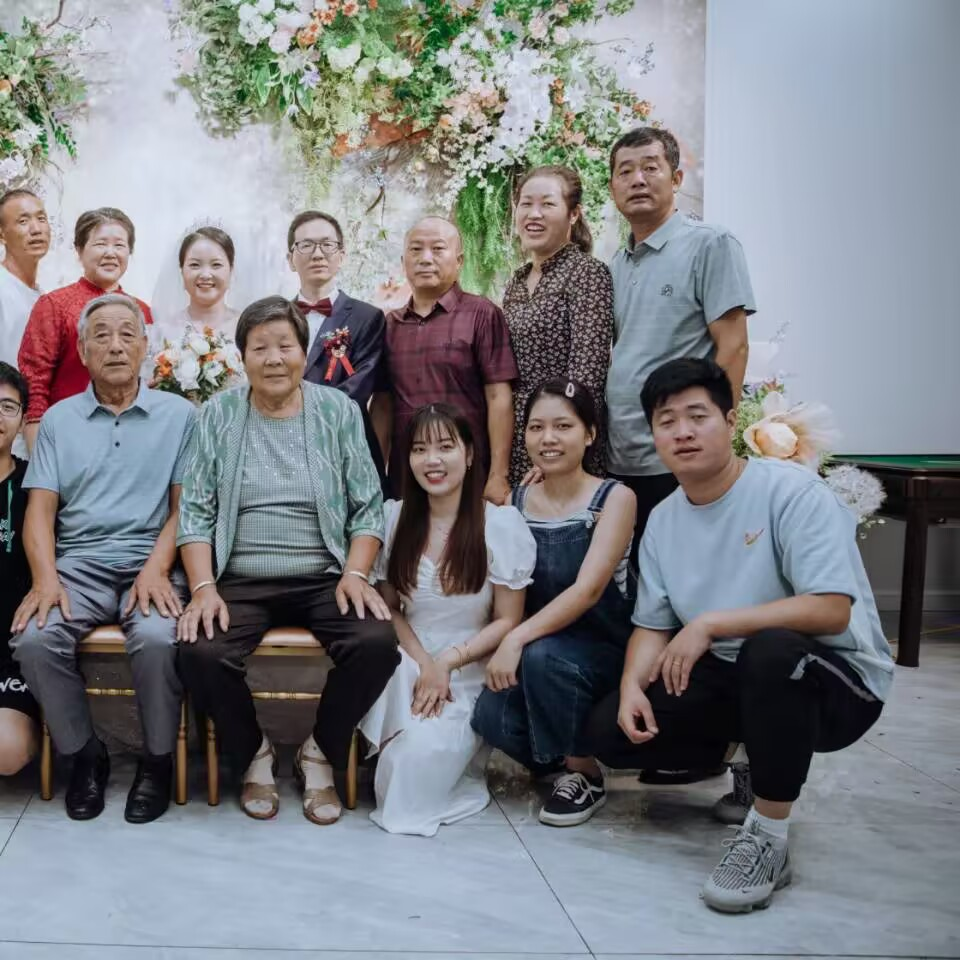
\includegraphics[width=\textwidth]{./Image/image1.1.jpg}
        \caption{测试素材1.1}
        \label{fig:img1.1}
    \end{subfigure}
    \hfill
    \begin{subfigure}{0.45\textwidth}
        \centering
        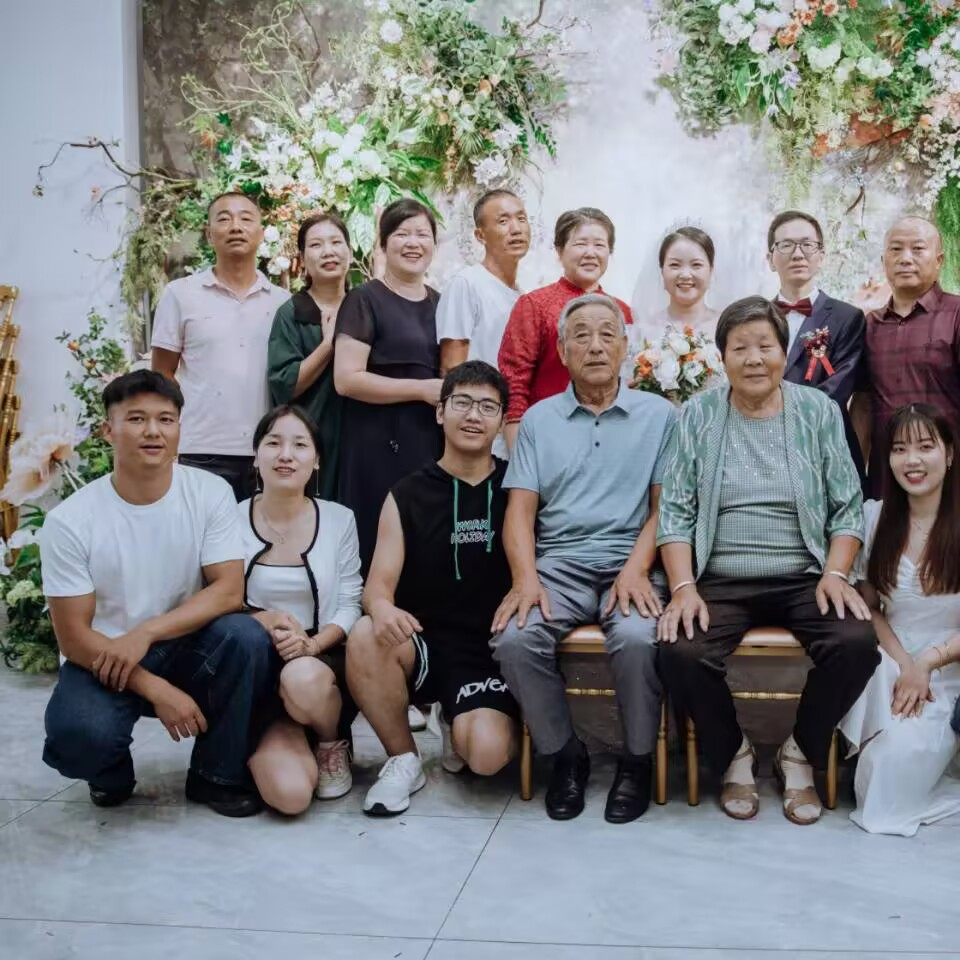
\includegraphics[width=\textwidth]{./Image/image1.2.jpg}
        \caption{测试素材1.2}
        \label{fig:img1.2}
    \end{subfigure}

    \caption{测试素材1}
    \label{fig:pair1}
\end{figure}

\begin{figure}[htbp]
    \centering

    \begin{subfigure}{0.45\textwidth}
        \centering
        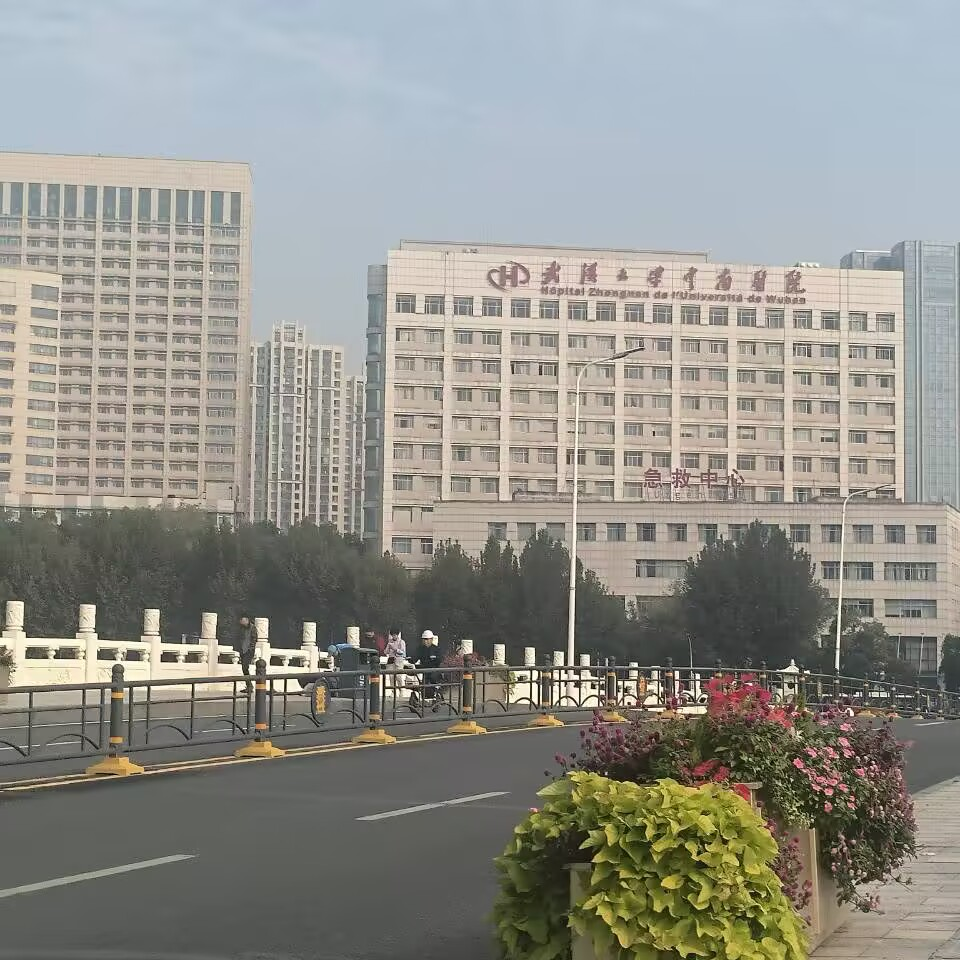
\includegraphics[width=\textwidth]{./Image/image2.1.jpg}
        \caption{测试素材2.1}
        \label{fig:img2.1}
    \end{subfigure}
    \hfill
    \begin{subfigure}{0.45\textwidth}
        \centering
        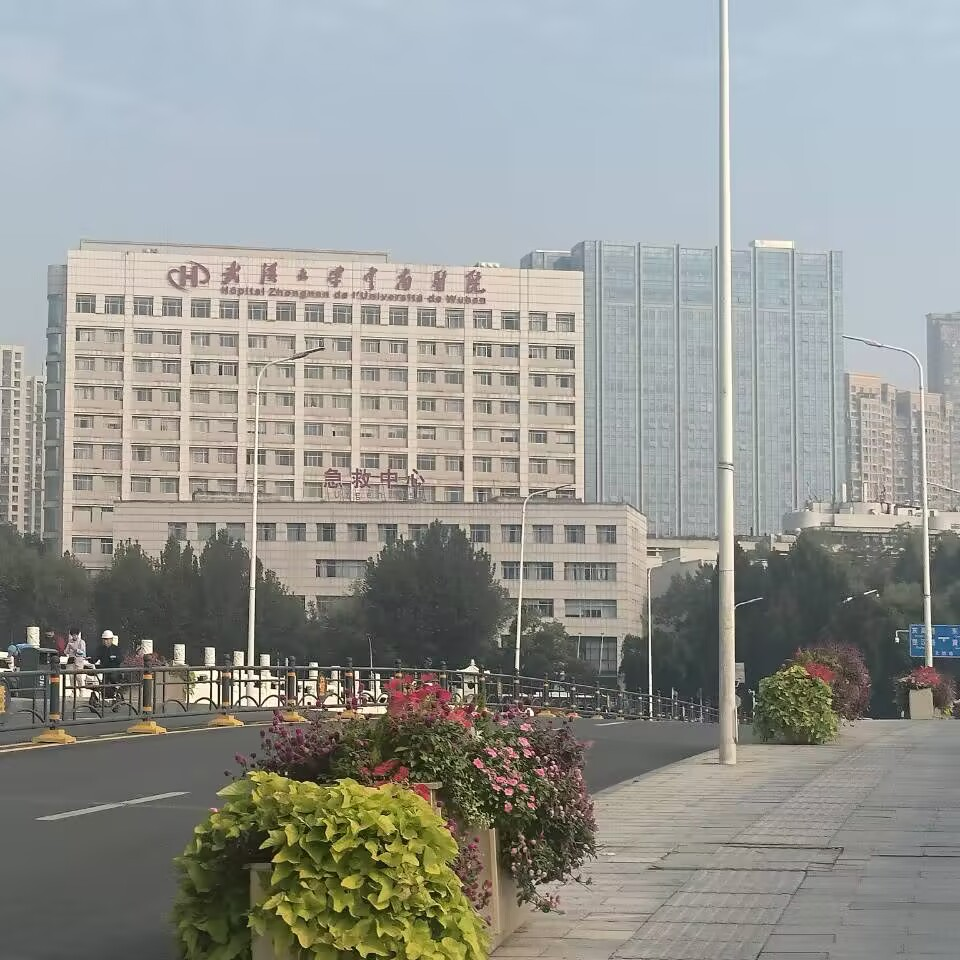
\includegraphics[width=\textwidth]{./Image/image2.2.jpg}
        \caption{测试素材2.2}
        \label{fig:img2.2}
    \end{subfigure}

    \caption{测试素材2}
    \label{fig:pair2}
\end{figure}

\subsection{结果展示}
结果如下:
\begin{figure}[htbp] 
	\centering 
	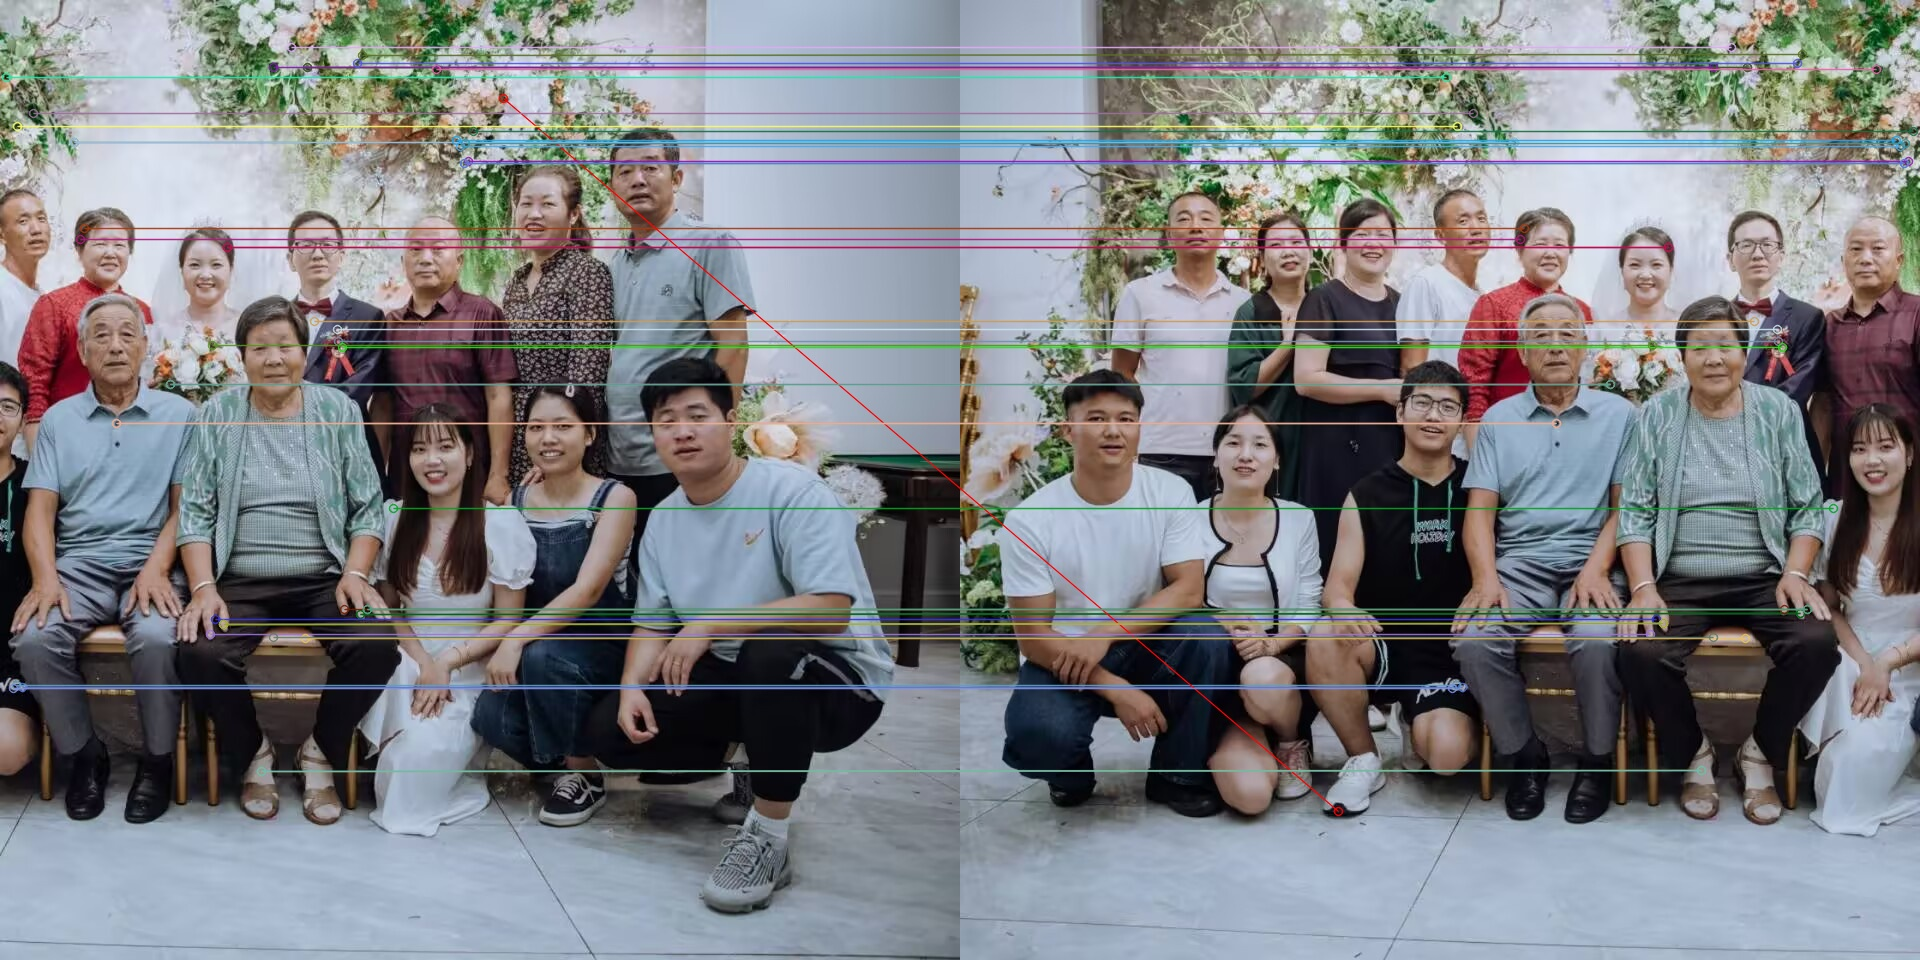
\includegraphics[width=0.8\textwidth]{./result/matches_visualization1.jpg} 
	\caption{测试素材1的特征匹配可视化结果} 
	\label{fig:result1.1} 
\end{figure}
\begin{figure}[htbp] 
	\centering 
	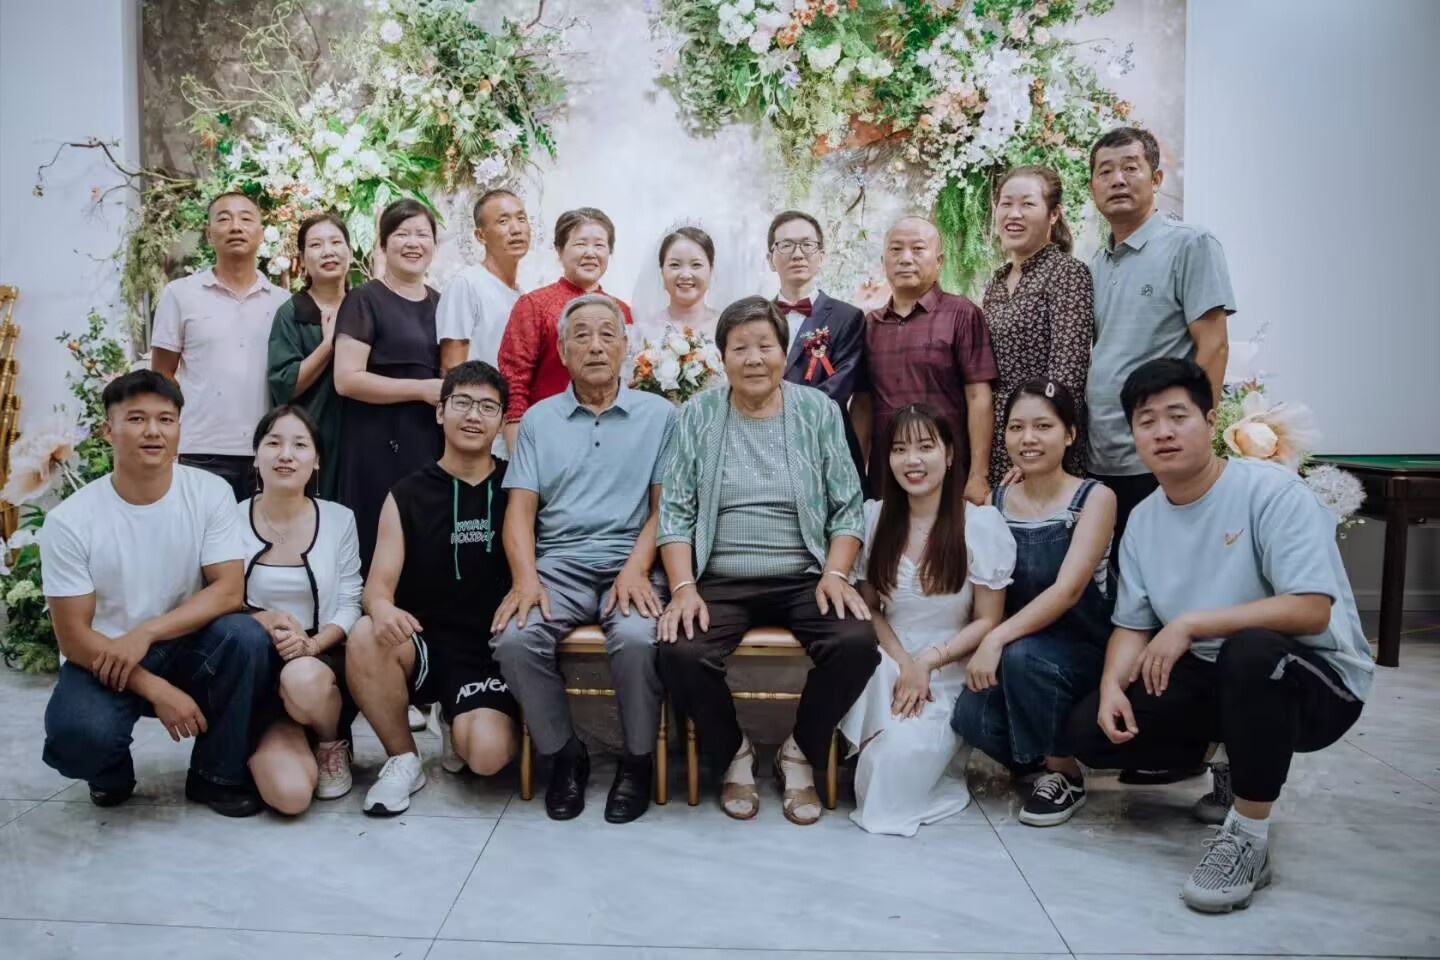
\includegraphics[width=0.6\textwidth]{./result/panorama_result1.jpg} 
	\caption{测试素材1的拼接可视化结果} 
	\label{fig:result1.2} 
\end{figure}
\begin{figure}[htbp] 
	\centering 
	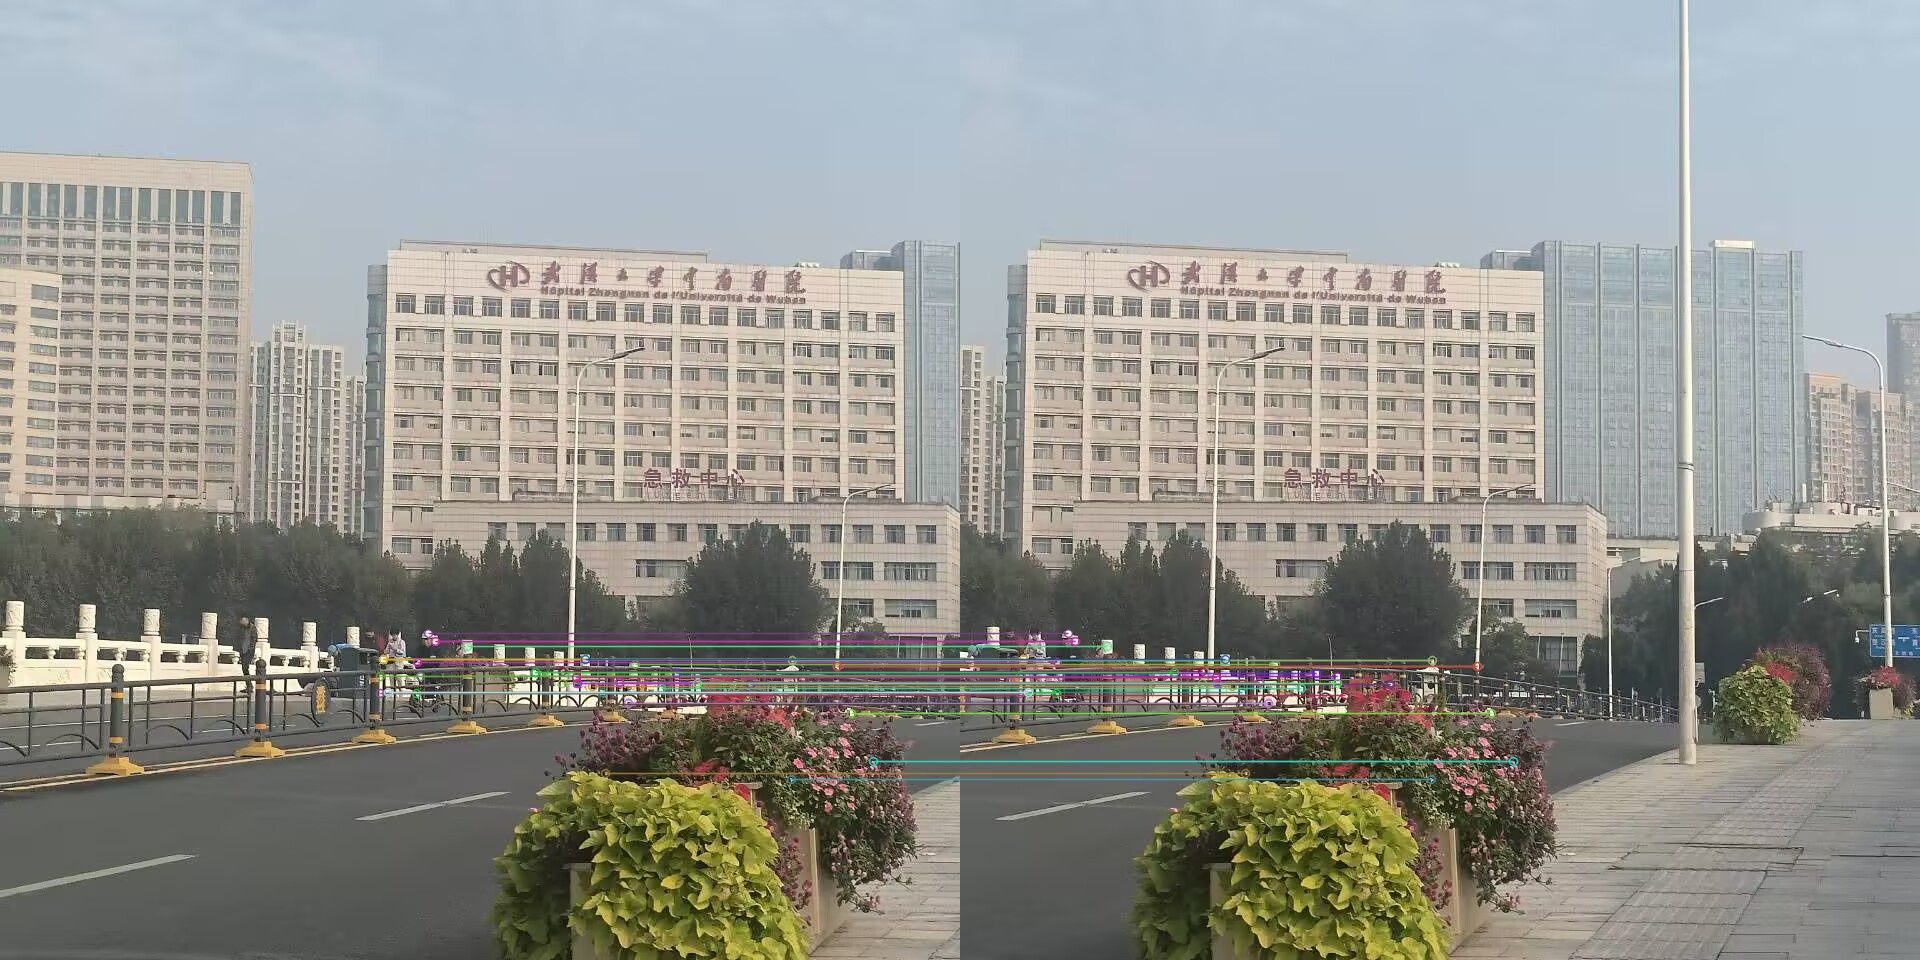
\includegraphics[width=0.8\textwidth]{./result/matches_visualization2.jpg} 
	\caption{测试素材2的特征匹配可视化结果} 
	\label{fig:result2.1} 
\end{figure}
\begin{figure}[htbp] 
	\centering 
	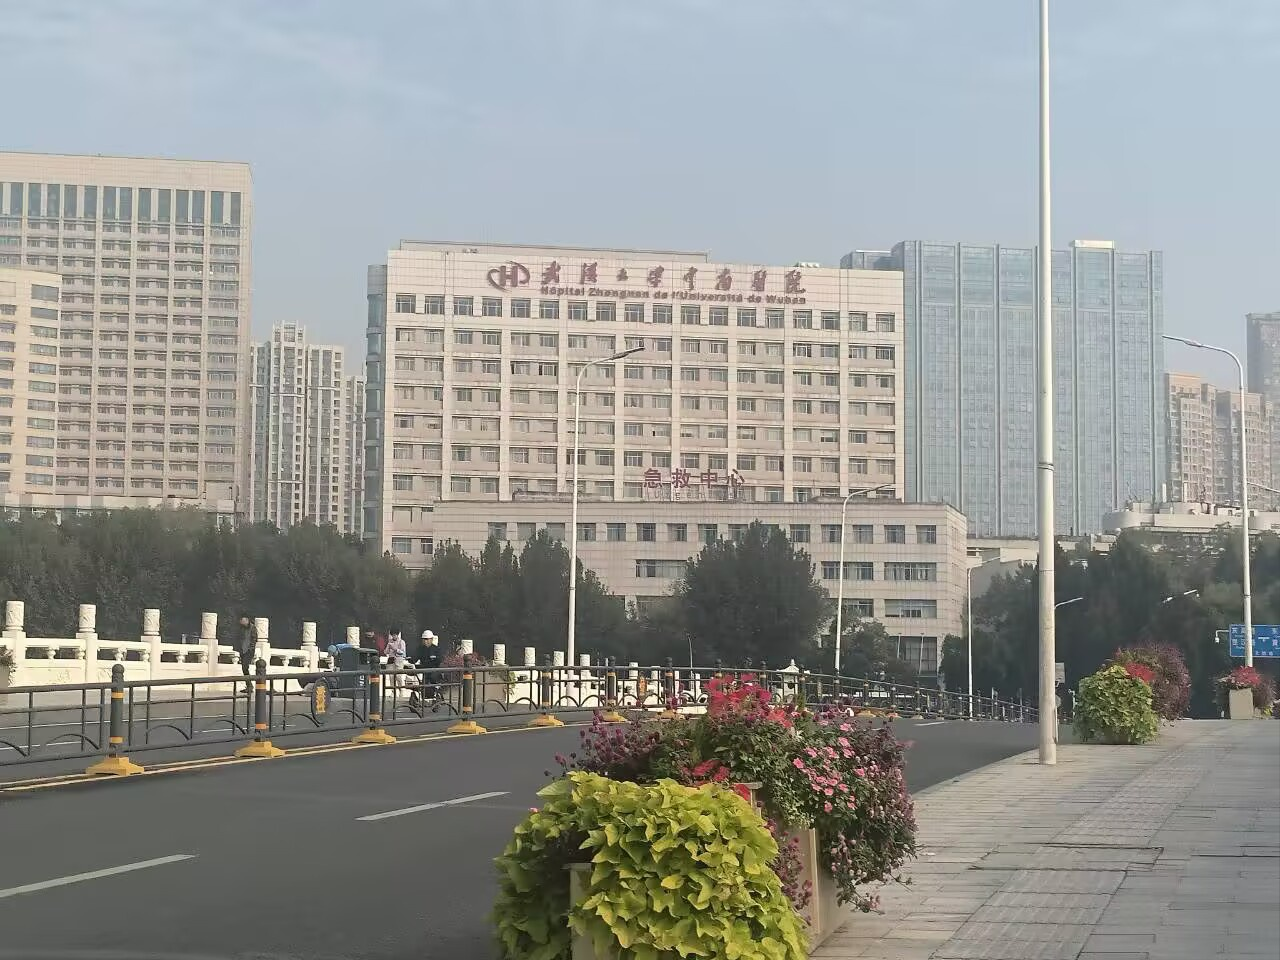
\includegraphics[width=0.6\textwidth]{./result/panorama_result2.jpg} 
	\caption{测试素材2的拼接可视化结果} 
	\label{fig:result2.2} 
\end{figure}
\subsection{结果分析}
从测试结果可以看出，所实现的图像拼接算法能够较好地完成全景图的生成任务。值得注意的是，测试素材1由于图像的特殊性，得到的显著的50组匹配点中
存在一组错误的匹配点（反映在图3中），但是在RANSAC算法的作用下，这些错误匹配点被成功剔除，保证了单应性矩阵估计的准确性，从而实现了较为理想
的拼接效果。
% 参考资料
\begin{thebibliography}{99}
\bibitem{ref1} 徐弘祯,李世超,季宇寒,等.基于特征点匹配的全景相机图像拼接方法研究[J].农业机械学报,2019,50(S1):150-158.
\bibitem{ref2} 柳运波.全景图像拼接关键技术研究[D].电子科技大学,2013.
\end{thebibliography}

\end{document}